%\documentclass[conference]{IEEEtran}
%\IEEEoverridecommandlockouts
\documentclass{article}
\usepackage[utf8]{inputenc}
\usepackage[%
    left=1.0in,%
    right=1.0in,%
    top=1.0in,%
    bottom=1.0in,%
    paperheight=11in,%
    paperwidth=8.5in%
]{geometry}

% =======================
\usepackage{xeCJK}
\usepackage{amssymb}
\usepackage{amsmath}
\usepackage{amstext}
\usepackage{amsopn}
%\usepackage{algorithmic}
\usepackage{graphicx}
\usepackage{textcomp}
\usepackage{xcolor}

\usepackage{textcomp}

\usepackage{boxedminipage}
\usepackage{enumerate}
\usepackage{multirow}
\usepackage{url}
\usepackage{times}
\usepackage{version}
% \usepackage[pdftex]{graphicx}
\usepackage{epsfig}
\usepackage{epsf}
%\usepackage{graphics}
\usepackage{caption}
\usepackage{subfigure}
\usepackage{algorithm}
\usepackage{algpseudocode}
%\PassOptionsToPackage{bookmarks={false}}{hyperref}
%%%%%%%%%%%%
\usepackage{comment}
\usepackage{multicol}
\usepackage{booktabs}
\usepackage{dblfloatfix}
\usepackage{listings}
\usepackage{xparse}
\usepackage{hyperref}
\usepackage{lmodern}
\usepackage{enumitem}
\lstset{language=C,keywordstyle={\bfseries \color{blue}}}

\input macro.tex
% ==========================

\setCJKmainfont[Path=fonts/]{msjh.ttc} % 中文字型
\setCJKmonofont[Path=fonts/]{msjh.ttc} % 中文等寬字型

\hypersetup{colorlinks=true, linkcolor=blue}

\begin{document}

\title{Group 4: E-Healthcare Management System}
\author{
  Cheng-Han Hsieh, 謝承翰\\
  \texttt{B103040012}
  \and
  Shih Yu Sun, 孫世諭\\
  \texttt{B103040001}
  \and
  Casper Liu, 劉世文\\
  \texttt{B093040051}
  \and
  Tina Tsou, 鄒宜庭\\
  \texttt{B096060032}
  \and
  Chia-Yen Huang, 黃嘉彥\\
  \texttt{B103040051}
  \and
  Ting-Hao Hsu, 許廷豪\\
  \texttt{B103040008}
}

\maketitle

\section{Outline}
\label{sec:outline}

  \begin{figure}[ht]
    \centering
    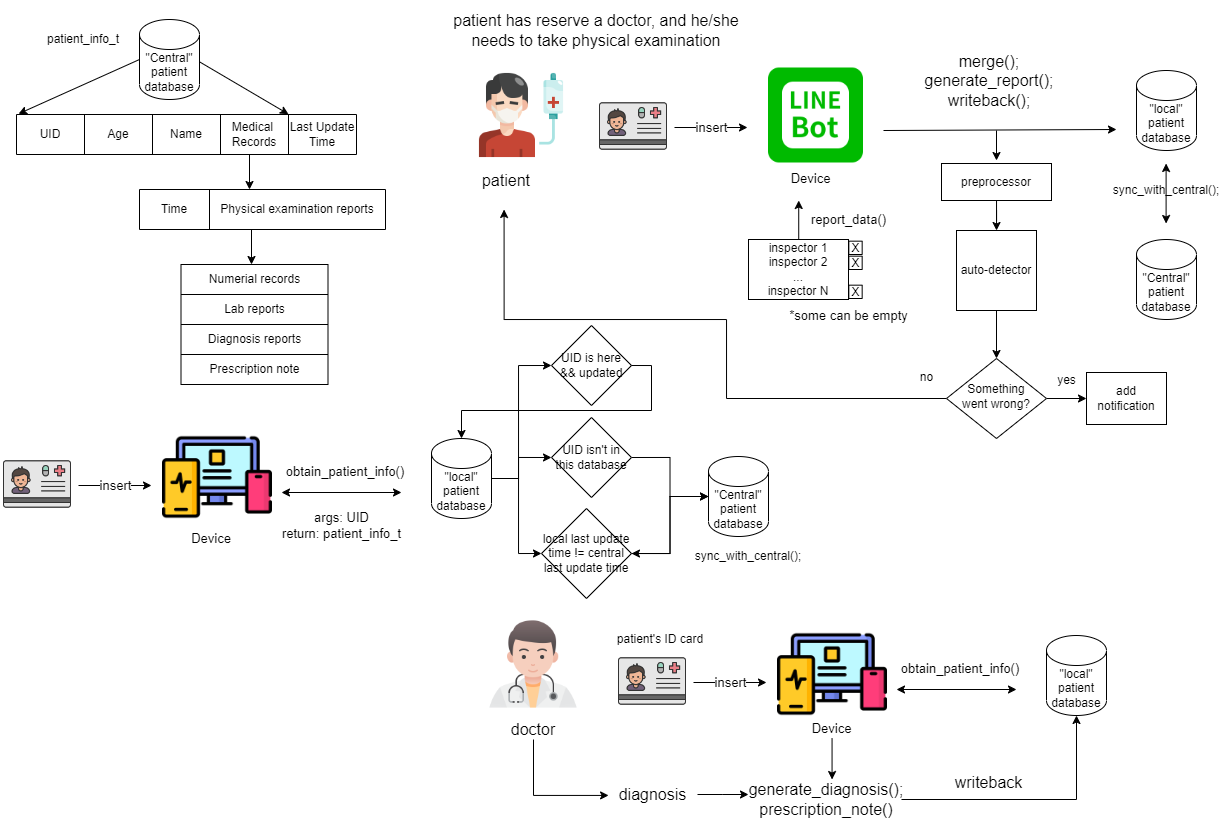
\includegraphics[scale = 0.25]{asset/flowchart.png}
    \caption{A simple example of outline.}
    \label{fig:flowchart}
  \end{figure}

  \xfig{fig:flowchart} shows the skelton of the whole system. The left-top 
  part is the scrawled database, which defines ``what'' is in the database. 
  As shown, the database contains necessary medical information of patients. 
  The right-top part is the situation that a patient has maken an appointment 
  with doctor and he need to take a physical examination first. By insert the 
  ID card, the physical data will be recorded into the local database, syncing 
  with the central database, and in the mean time, the result of examination 
  will be sended to ``auto-detectors'', which detect the abnormal data in the 
  physical reports, and notify the patient. The auto-detectors can detect 
  potential diseases like cancer by determining the gene expression profiling, 
  or diabetes by the physical data. 
  The middle part is the situation that a patient or a doctor wants to obtain 
  the information of the patient. After inserting the ID card, the local 
  database will check whether the status of corresponding data. If it is out of 
  date or not exists, the local database will try to sync with the central 
  database, otherwise create a new one if this patient is totally new. Eventually, 
  the information of this patient is returned to the client (device). 
  The bottom part shows a doctor make the diagnosis and prescription for the 
  patient. The new diagnosis and prescription are write-backed to the local 
  database, and also sync with the central one. 

\section{Features}
\label{sec:features}

  With this E-healthcare management system, the hospital/clinic can easily 
  sync the information of patients with other health systems, manage 
  the information of patients.
  For patients, the patient can do most of the things online, for example, 
  make a doctor appointment, look up the medical records and prescriptions, 
  and obtain the physical reports at home. Even more, the system use machine 
  learning to detect the abnormal data in the reports, notify the patient 
  to prevent the disease becoming worse. 
  To conclusion, the major features of the system can be summarized as 
  followings: 
  \begin{itemize}
    \item Automatically sync the information of patients between different health systems by using local and central database. 
    \item Facilitate the accessing of medical records and prescriptions, for both doctors and patients. 
    \item Introduce the automatic disease detectors by leveraging machine learning and big data. 
  \end{itemize}

\section{Methodology}
\label{sec:methodology}
  \subsection*{Database}
  \begin{figure}[ht]
    \centering
    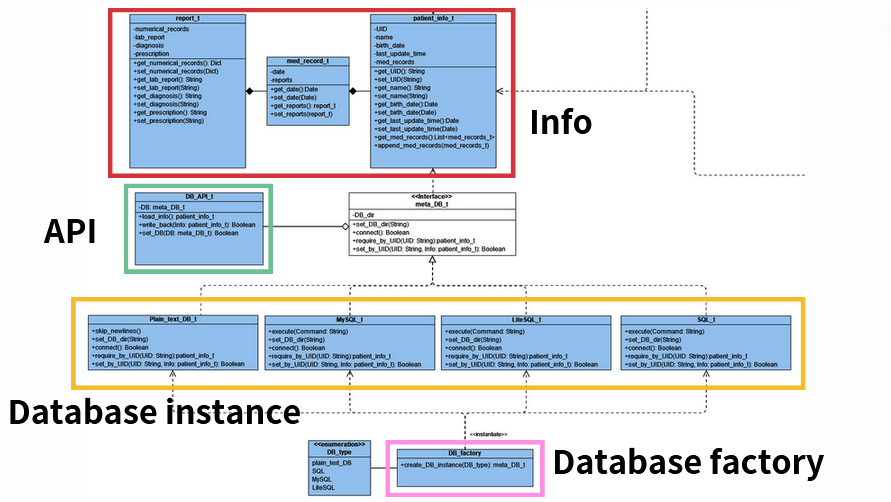
\includegraphics[scale = 0.6]{asset/database/DB_UML.png}
    \caption{The UML of the whole database.}
    \label{fig:DB_UML}
  \end{figure}
  \xfig{fig:DB_UML} shows the UML of the database. It can be divided into four 
  parts, the class definition of patients' information, the database API, the 
  class definition of database, and the database factory. 

  \begin{figure}[ht]
    \centering
    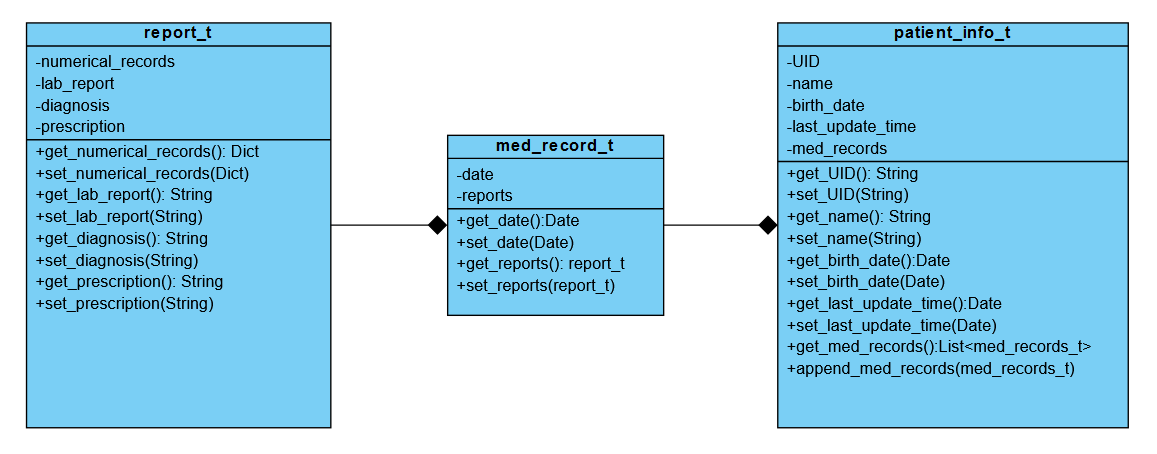
\includegraphics[scale = 0.35]{asset/database/pinfo.png}
    \caption{The UML of the class definition of patient information.}
    \label{fig:pinfo_UML}
  \end{figure}
  \xfig{fig:pinfo_UML} shows the class definition of the patients' information. 
  The class, \codeword{patient\_info\_t}, contains the necessary information of 
  a patient, for example, UID, name, birth date, and the list of medical records. 
  And in the class, \codeword{med\_record\_t}, is date and reports, like diagnosis, 
  prescriptions, and physical data and reports. 
  In this part, it provides a definition of patients' information for the whole 
  database. Later, the database will depend on the class defined in this part. 

  \begin{figure}[ht]
    \centering
    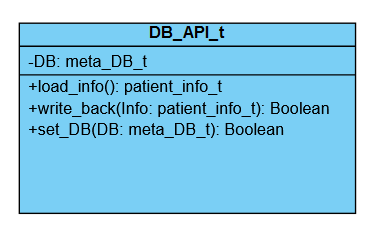
\includegraphics[scale = 0.5]{asset/database/DB_API.png}
    \caption{The UML of the class definition of database API.}
    \label{fig:API_UML}
  \end{figure}
  \xfig{fig:API_UML} is the definition of the API of the database. It provide 
  some simple and secure methods to access the database, for example, load the 
  information of a patient, update the information, and set the database. 
  Later, those parts of the system that need to access the database rely on 
  this API. 

  \begin{figure}[ht]
    \centering
    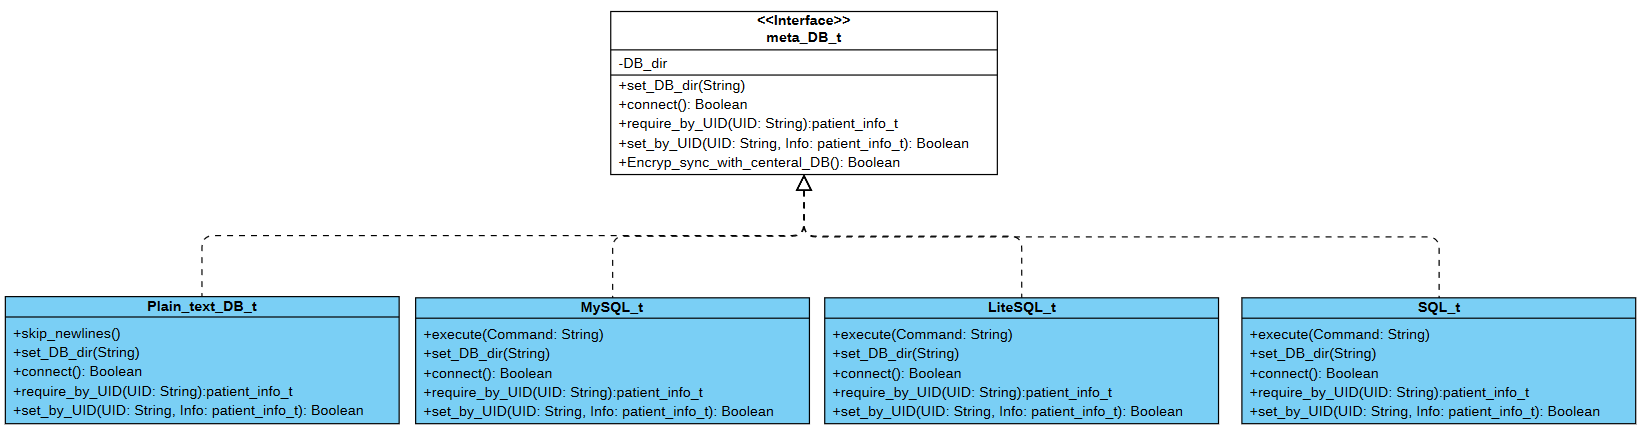
\includegraphics[scale = 0.5]{asset/database/database_instance.png}
    \caption{The UML of the class definition of database instance.}
    \label{fig:DB_instance}
  \end{figure}
  Here is the definition of the databases. First is an interface of the 
  database, it defines some common methods of database, like connect, require, 
  update, and sync with other database. 
  Then are the specialized databases. Here, plain text database, SQLs are defined. 

  The rationales behind the need of an interface is, in the early development, 
  we did not determine which type of database should be use. And second, when 
  scaling the system up, the database may need to be replaced with other databases 
  that have higher throughput and lower response time, like ScyllaDB. 
  An interface of the database solves the problems, because it abstracts the 
  database and unify the methods. The additional databases can be easily provided 
  by following the interface. 

  \begin{figure}[ht]
    \centering
    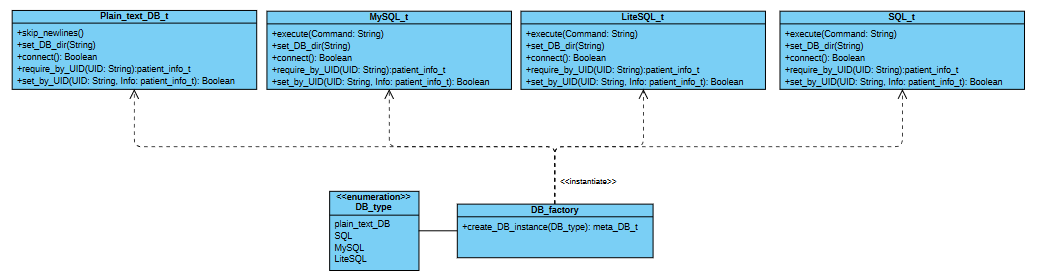
\includegraphics[scale = 0.7]{asset/database/factory_UML.png}
    \caption{The UML of the factory of databases.}
    \label{fig:factory_UML}
  \end{figure}

  \begin{figure}[ht]
    \centering
    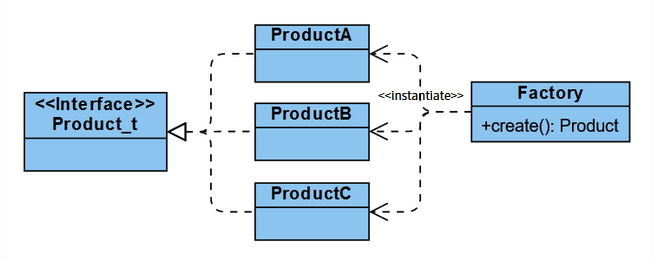
\includegraphics[scale = 0.5]{asset/database/simple_factory.png}
    \caption{The UML of a simple factory.}
    \label{fig:simple_factory}
  \end{figure}
  Then is the factory of database, which shown in \xfig{fig:factory_UML}. 
  In short, factory is responsible for instantiating the database. And it is actually 
  a pattern from $\textit{Design Patterns}$. 
  The general UML of factory pattern is shown in \xfig{fig:simple_factory}. The 
  products inherit a common interface, and they are all instantiated by the factory. 
  The advantage of factory patterns is it hides the details of ``creation'', which 
  allows the factory changing the implementation without modifying the usage of the 
  creation. It is a very import characteristics in developing a big system. The 
  modification of the usage of methods can cost lots of time and effort, because 
  all the programs that use the methods should be modified. 
  
  To conclusion, this design of database has the following features:
  \begin{itemize}
    \item Hide the detail of the creation. 
    \item An uniform application interface. 
    \item High Scalability. 
    \item Easy to maintain. 
  \end{itemize}

%\section{Code}
%\label{sec:code}

\subsection*{Frontend and Medium}

\begin{figure}[ht]
  \centering
  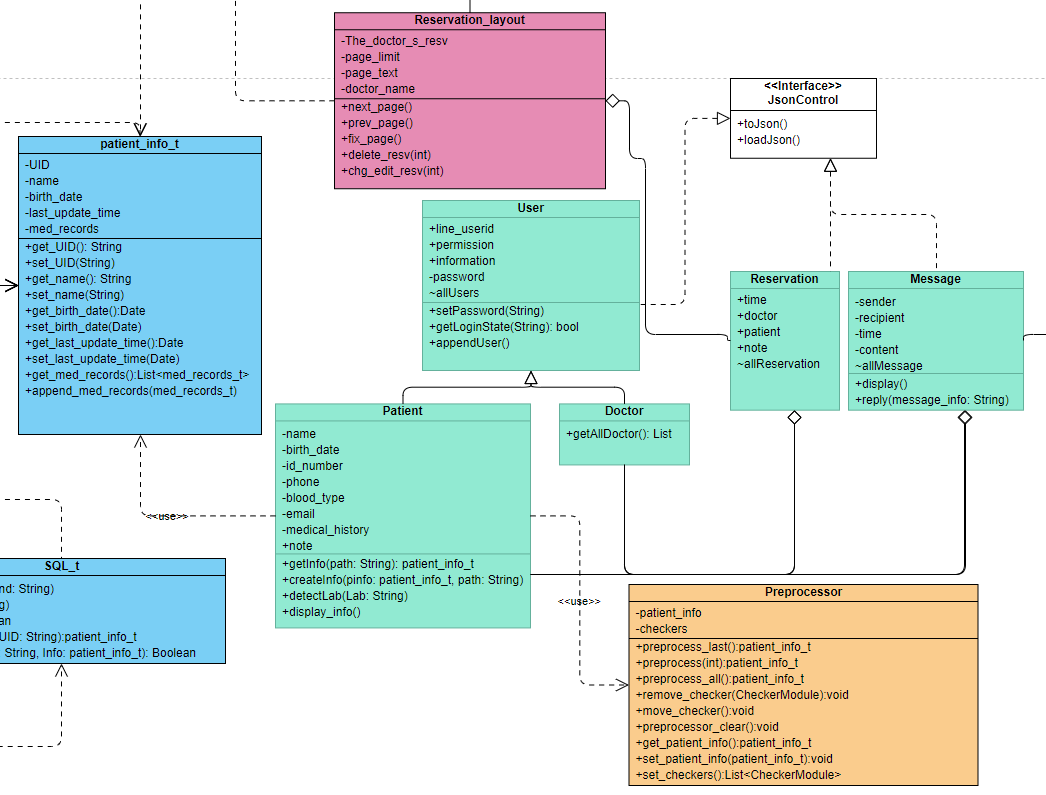
\includegraphics[scale = 0.45]{asset/frontend_and_medium/MED_whole.png}
  \caption{The UML of frontend and medium.}
  \label{fig:uml_frontend_and_medium}
\end{figure}

In the code for the patient frontend and middleware, our functionalities 
are as follows (refer to Figure \ref{fig:uml_frontend_and_medium}):

\begin{enumerate}[label=\arabic*.]
    \item Utilize Ngrok to forward external requests to the locally specified port.
    \item Integrate LineBot, HTML, JS, and CSS, serving as the patient frontend to send requests such as registration, message sending, and reservations.
    \item Connect to the database to retrieve detailed information based on the user's ID.
    \item Interface with the Processor (Lab), sending detailed information retrieved from the database to the C++ Processor (Lab) for processing and receiving the information back.
    \item Enable the Doctor GUI to utilize the Patient Class to 
    \begin{enumerate}[label=(\roman*)]
        \item obtain detailed information from the database,
        \item access return information from the Processor (Lab),
        \item retrieve the Message Class, and
        \item use the \codeword{Reply()} method to quickly respond to messages via LineBot (refer to Figure \ref{fig:uml_frontend_and_medium}),
        \item obtain detailed data from the Reservation Class,
        \item access the Doctor Class, and
        \item verify its name and password for login.
    \end{enumerate}
\end{enumerate}

Next, we will explain each class in the frontend and 
medium, highlighting some special member functions and 
attributes:

\subsubsection*{User}

\begin{itemize}
    \item An abstract class primarily responsible for handling account information such as:
    \begin{enumerate}[label=(\roman*)]
        \item \codeword{permission:} Manages permissions, used to confirm the current user mode (admin or guest).
        \item \codeword{line\_id:} Mainly used to record the user's Line ID, this information is automatically obtained from Line during registration and transmitted to our server.
        \item \codeword{getLoginState(String):} Takes a password as input and checks if it is the correct password.
    \end{enumerate}
\end{itemize}

\subsubsection*{Patient}

\begin{itemize}
    \item A child class of User, mainly deals with patient account information, where it interfaces with the \codeword{patient\_info\_t} in the database to obtain detailed data such as heart rate, blood glucose:
    \begin{enumerate}[label=(\roman*)]
        \item \codeword{detectLab(String):} Will send the information of \codeword{patient\_info\_t} to the Preprocessor, obtaining a detailed diagnosis such as "high heart rate," "diabetes risk," etc (refer to Figure \ref{fig:uml_medium_preprocessor_database}).
    \end{enumerate}
\end{itemize}

\begin{figure}[ht]
  \centering
  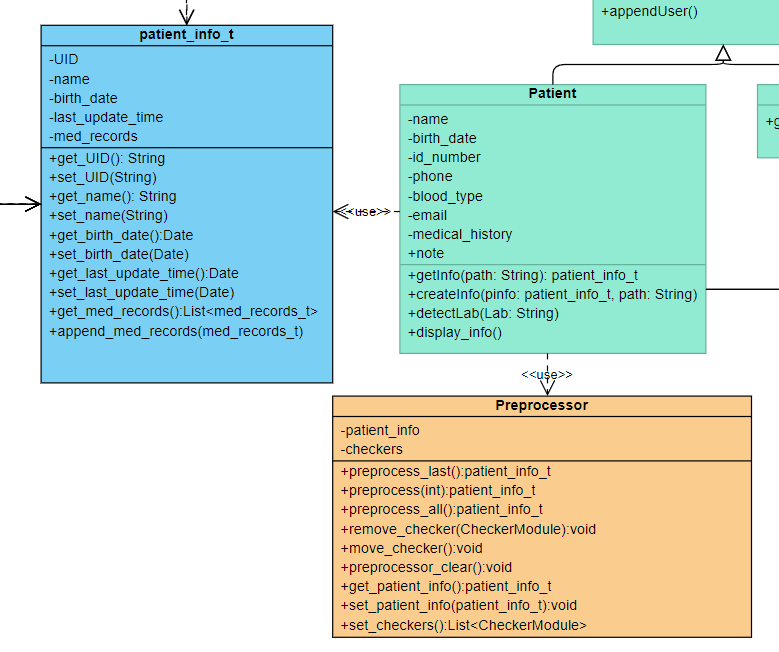
\includegraphics[scale = 0.35]{asset/frontend_and_medium/MED_usage_processor_DB.png}
  \caption{The UML of interaction between medium, preprocessor and database.}
  \label{fig:uml_medium_preprocessor_database}
\end{figure}

\subsubsection*{JsonControl}

\begin{itemize}
    \item An interface implemented by the User, Reservation, and Message classes. Its main purpose is to serialize objects into JSON files for easy storage and access:
    \begin{enumerate}[label=(\roman*)]
        \item \codeword{toJson():} Stores all objects of the entire class in JSON format.
        \item \codeword{loadJson():} Reads a JSON file and restores all objects from it into a list.
    \end{enumerate}
\end{itemize}

\subsubsection*{Reservation}

\begin{itemize}
    \item When a patient uses the frontend LineBot to make a reservation, a Reservation object is created. It is used and deleted by the Doctor GUI and includes Patient and Doctor objects to determine the patient and the reserved doctor (refer to Figure \ref{fig:uml_medium_and_doctor_gui}).
\end{itemize}

\subsubsection*{Message}

\begin{itemize}
    \item When a patient uses the frontend LineBot to send a message, a Message object is created. It is used, replied to, and deleted by the Doctor GUI and includes Patient and Doctor objects to determine the patient and the doctor being messaged (refer to Figure \ref{fig:uml_medium_and_doctor_gui}):
    \begin{enumerate}[label=(\roman*)]
        \item \codeword{reply():} Based on its own Patient object, it uses LineBot to send a message back to the patient (because the Patient object contains the line\_id attribute).
    \end{enumerate}
\end{itemize}

\begin{figure}[ht]
  \centering
  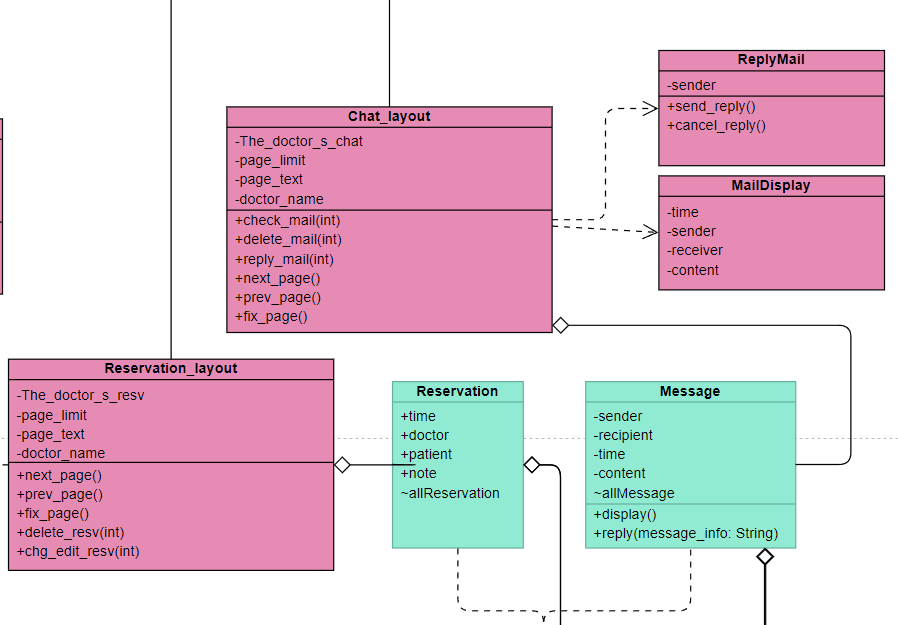
\includegraphics[scale = 0.35]{asset/frontend_and_medium/MED_usage_doctor_gui.png}
  \caption{The UML of interaction between medium and Doctor GUI.}
  \label{fig:uml_medium_and_doctor_gui}
\end{figure}

\subsubsection*{Preprocessor}

\begin{itemize}
    \item  The preprocessor is created with its checkers made with CheckerModule. Before any kind of preprocessor is created, one or more checkers should be created first by the programmer. The programmer should create checker based on the demand from the dotcor and under the rule of ChckerModule. The preprocessor is useful to preprocess the data, like fixing the wrong data based on the right data and existing formula, or deleting the NAN data and so on. Input the data into the preprocessor's preprocessing-specific function, data then be preprocessed. Modify or add the checker(s) into the preprocessor with checker-modifying function. When the data is preprocessed, the programmer can assume those data ready for detecting in the next part: Detector.(refer to Figure \ref{fig:pre_preprocessor}):
    \begin{enumerate}[label=(\roman*)]
        \item \codeword{preprocess\_last():} Preprocess the data in the last and newest profile stored in patient\_info.
        \item \codeword{preprocess(x):} Preprocess the data the no.\codeword{x} profile stored in patient\_info.
        \item \codeword{preprocess\_all():} Preprocess the data of all profiles stored in patient\_info.
        \item \codeword{move\_checker(x):} Move the new checker "\codeword{x}" into the preprocessor.
        \item \codeword{remove\_checker():} Remove the last moved checker from the preprocessor.
        \item \codeword{clear\_checker():} Clear all the checkers from the preprocessor.
    \end{enumerate}
\end{itemize}

\begin{figure}[ht]
  \centering
  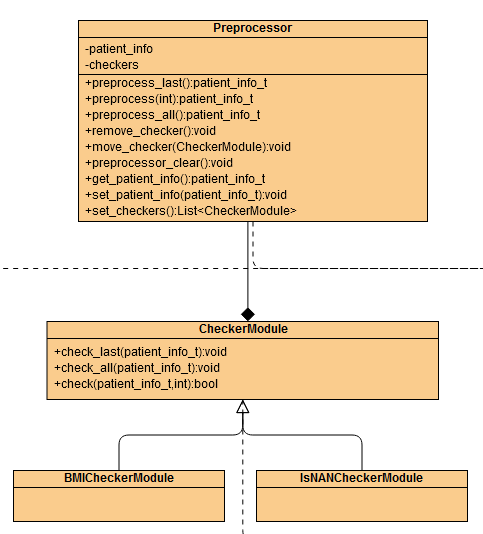
\includegraphics[scale = 0.35]{asset/preprocessor_and_detector/PRE_preprocessor.png}
  \caption{The UML of preprocessor and its composition: CheckerModule.}
  \label{fig:pre_preprocessor}
\end{figure}

\subsubsection*{Detector}
%The metadetector is created with its detectors made with DetectorModule. Before any kind of metadetector is created, one or more detectors should be created first by the programmer. 
\begin{itemize}
    \item The metadetector defined an uniform methods to detect abnormal data of physical data of a patient. Based on the demand from the dotcor, the corresponding specialized detector will be created, like \codeword{BMIDetectorModule} and \codeword{HeartRateDetectorModule}. The result can be obtained from Detector\_Status in a general way, or list of strings that contains detailed information to be used in more specific situation. (refer to Figure \ref{fig:pre_detector}):
    \begin{enumerate}[label=(\roman*)]
        \item \codeword{detect(Description,Status):} Detect the illness or abnormal value in the last and newest profile stored in patient\_info. \codeword{Description} contains list of string that stores more detailed information, and \codeword{Status} give an easy for programmer to verify the result. The detector do not support detecting for non-last profile, because it's without apparent cause.
        \item \codeword{move\_detector(x):} Move the new detector "\codeword{x}" into the meta-detector.
        \item \codeword{remove\_detector():} Remove the last moved detector from the meta-detector.
        \item \codeword{clear\_detector():} Clear all the detector from the meta-detector.
    \end{enumerate}
\end{itemize}
\begin{figure}[ht]
  \centering
  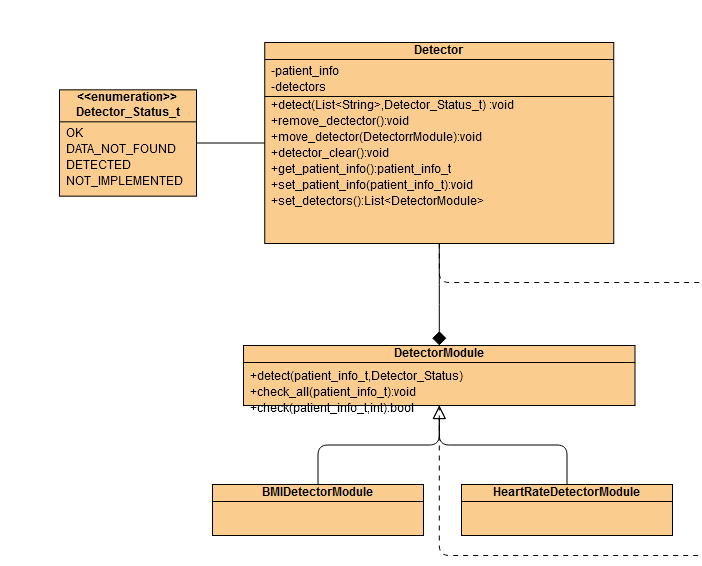
\includegraphics[scale = 0.35]{asset/preprocessor_and_detector/PRE_detector.png}
  \caption{The UML of detector and its composition: DetectorModule. The Detector\_status\_t is contained in the picture as well, which is used to present the status of the result.}
  \label{fig:pre_detector}
\end{figure}

\subsection*{Frontend(DoctorGUI)}

\begin{figure}[ht]
    \centering
    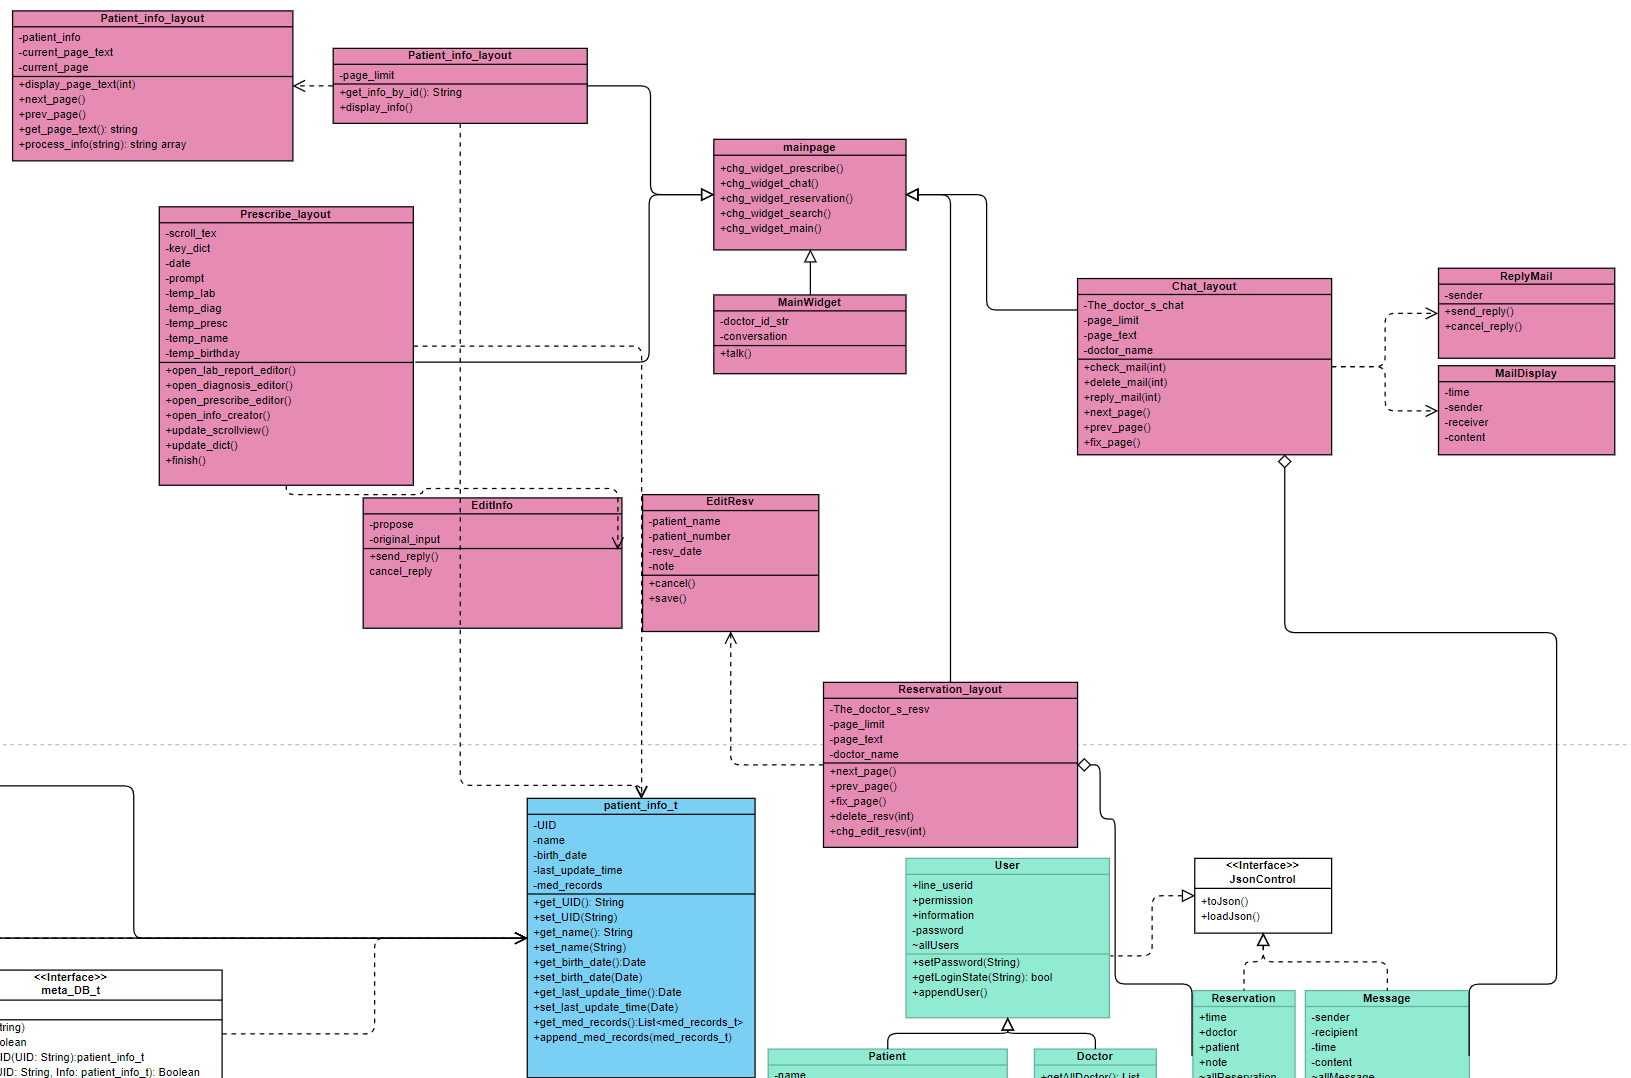
\includegraphics[scale = 0.3]{asset/doctor_gui/frontend_uml.png}
    \caption{The UML of frontend.}
    \label{fig:frontend_uml}
  \end{figure}

\subsubsection*{Abstract}
The frontend, also can be called Doctor GUI, provide doctors with complete medical consultation functions such as :

\begin{itemize}
    \item Viewing patient information
    \item Editing prescriptions
    \item Replying to patient messages
    \item Viewing and modifying patient reservation information
\end{itemize}

By using this system, doctors can overcome space and 
time constraints. In addition to communicating with 
patients and making appointments in a timely manner, 
they can also synchronize all doctors' information 
in a timely manner, so that patients do not have to 
re-establish files every time they go to a hospital.

The GUI mainly communicates with the database and 
medium (linebot), displays the data on the interface, 
and provides editing and deletion functions. 

%Next, I will explain in detail the method of each class and how they communicate with other classes.

\subsubsection*{MainWidget and Design}
\begin{figure}[ht]
    \centering
    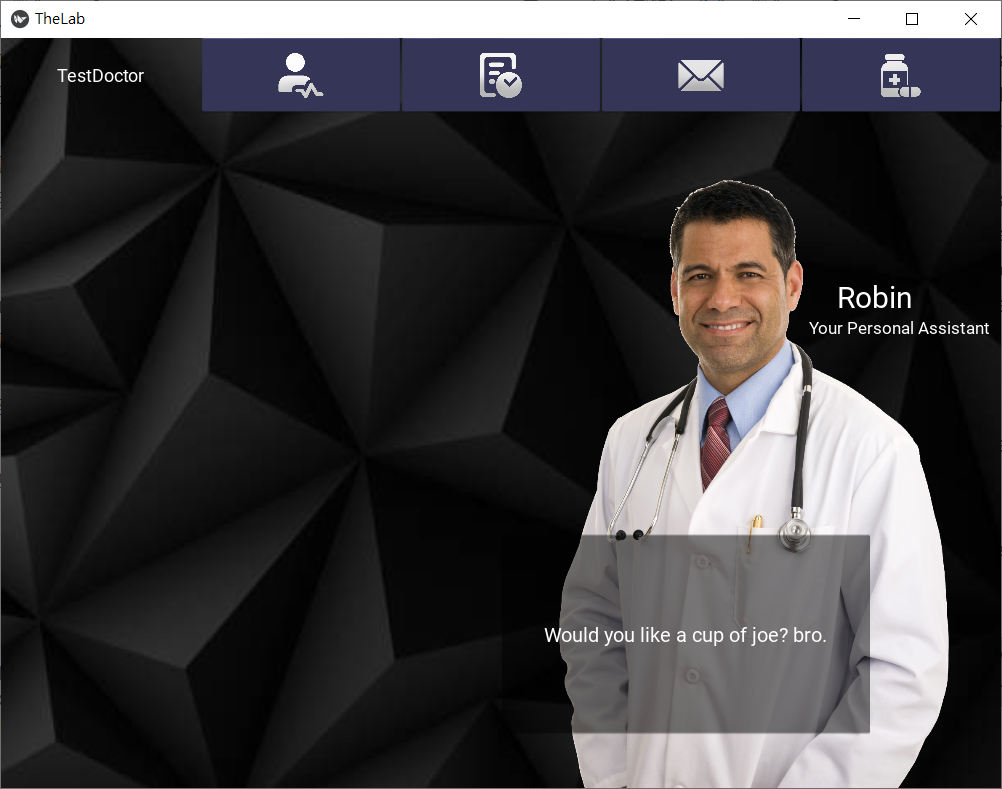
\includegraphics[scale = 0.35]{asset/doctor_gui/frontend_main.png}
    \caption{This is the preview of Mainwidget. The doctor will switch to this page after successfully logging in, which vaguely represents the general architecture design of the entire front-end.}
    \label{fig:frontend_main}
\end{figure}
\begin{itemize}
    \item There is a row of buttons at the top. Press to switch pages. These buttons exists on every main page, allowing doctors to jump more conveniently.
    \item There is a personal assistant in front of you. Press the dialog box and the assistant will talk to you. Currently, the conversations are random. If necessary in the future, you can communicate with other classes to implement functions similar to prompt notifications.
\end{itemize}

\subsubsection*{Mainpage}
mainpage is a class mainly provides the function of 
switching the page, allowing other pages to inherit 
and increase the reuse rate of the program.

\subsubsection*{Patient\_info\_layout}
%\begin{figure}[h]
%  \centering
%  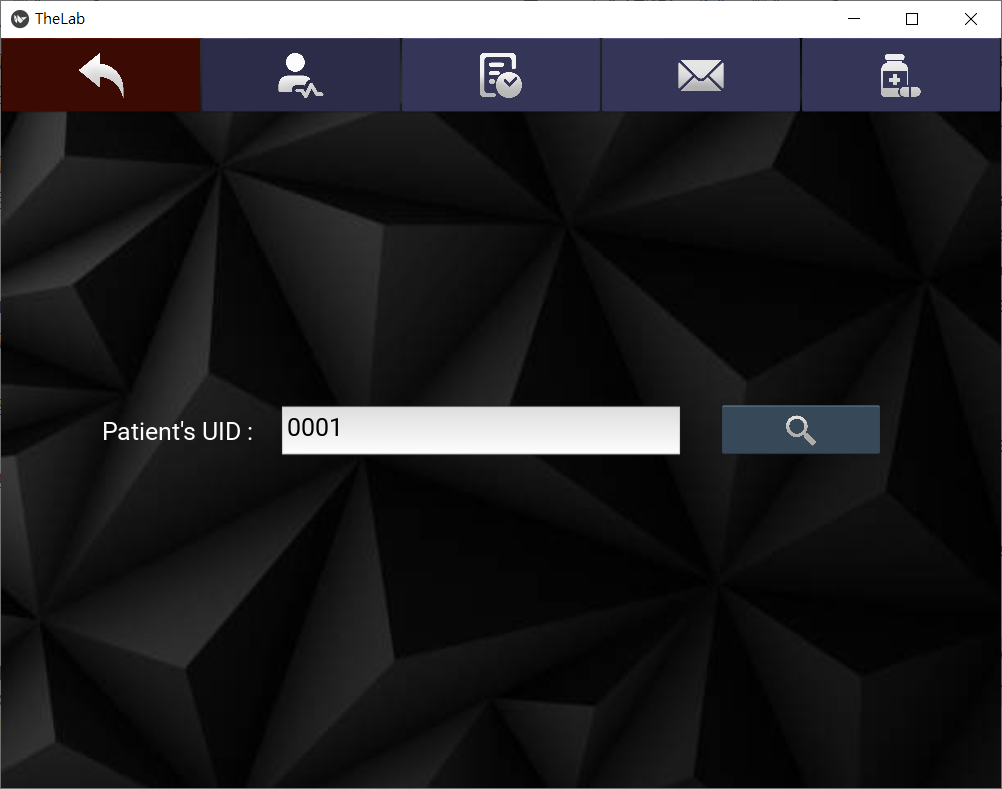
\includegraphics[scale = 0.4]{asset/doctor_gui/frontend_search_patient.png}
%  \caption{The prview of patient\_info\_layout}
%  \label{fig:frontend_search_patient}
%\end{figure}

\begin{figure*}[htb]
  \vspace{\baselineskip}
  \begin{center}
      \begin{tabular}{cc}
          \subfigure[]{\resizebox{0.4\textwidth}{!}{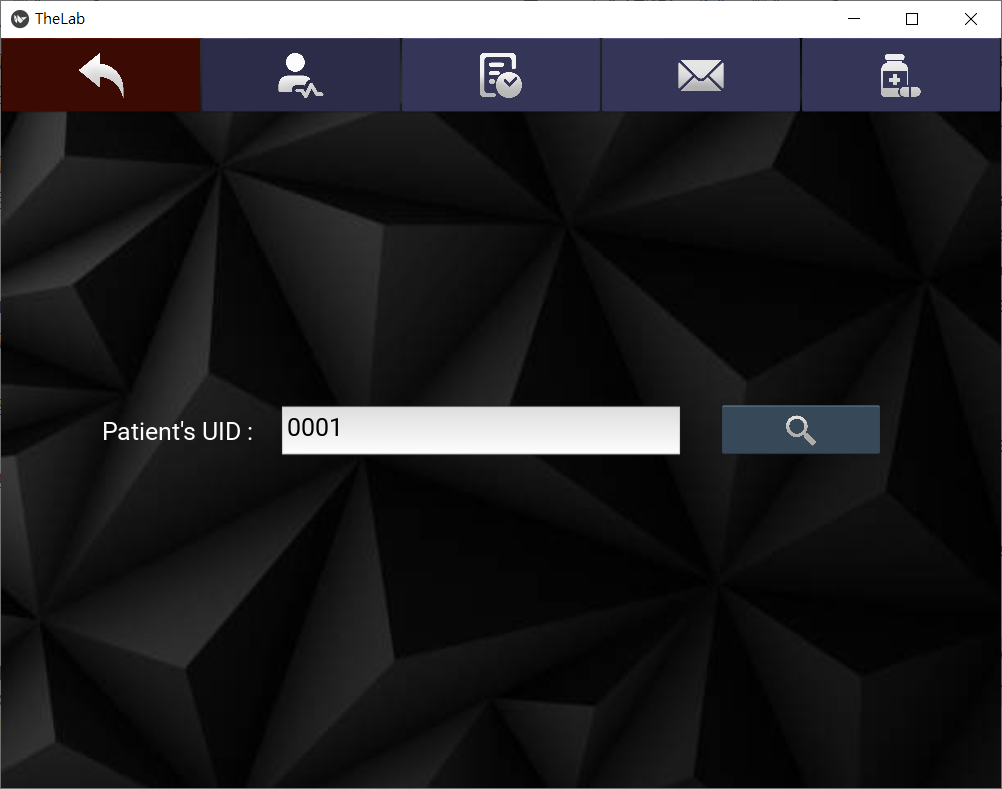
\includegraphics{asset/doctor_gui/frontend_search_patient.png}}}
          \subfigure[]{\resizebox{0.4\textwidth}{!}{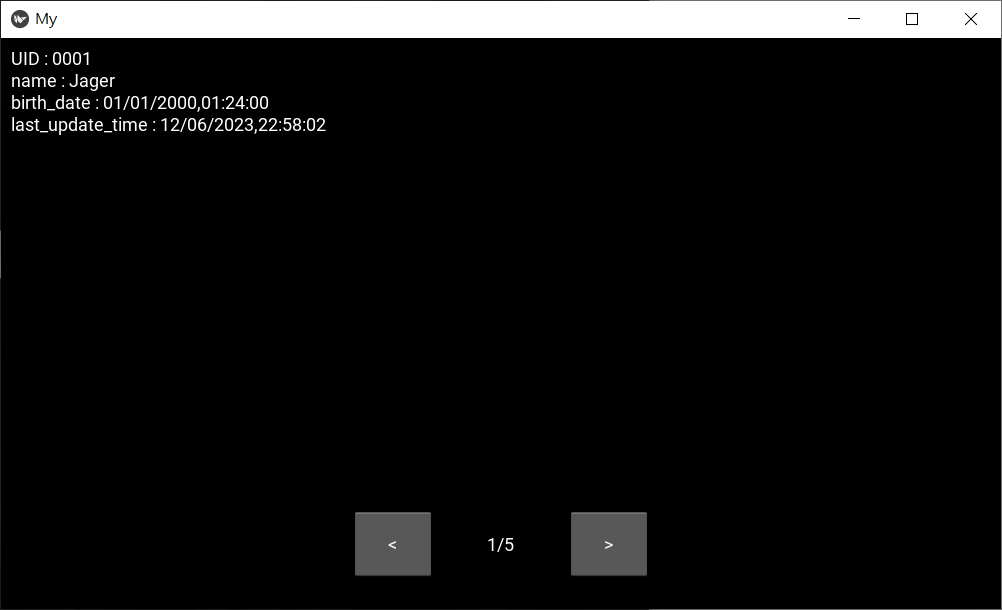
\includegraphics{asset/doctor_gui/frontend_patient_info.png}}}
      \end{tabular}
      \caption{(a) The prview of patient\_info\_layout 
      (b) The prview of describe object }
      \label{fig:frontend_patient_info}
  \end{center}
  \vspace{-\baselineskip}
\end{figure*}

The page firstly get input from textbox, and use 
\codeword{get\_info\_by\_id()} to call serials of methods in 
\codeword{patient\_info\_t} to load info of the patient the 
doctor wants to search. Then, it will call \codeword{display\_info()} 
to open a subprocess and pass the patient's info it gets. The 
subprocess can use a describe object to present these info.
%\begin{figure}[h]
%  \centering
%  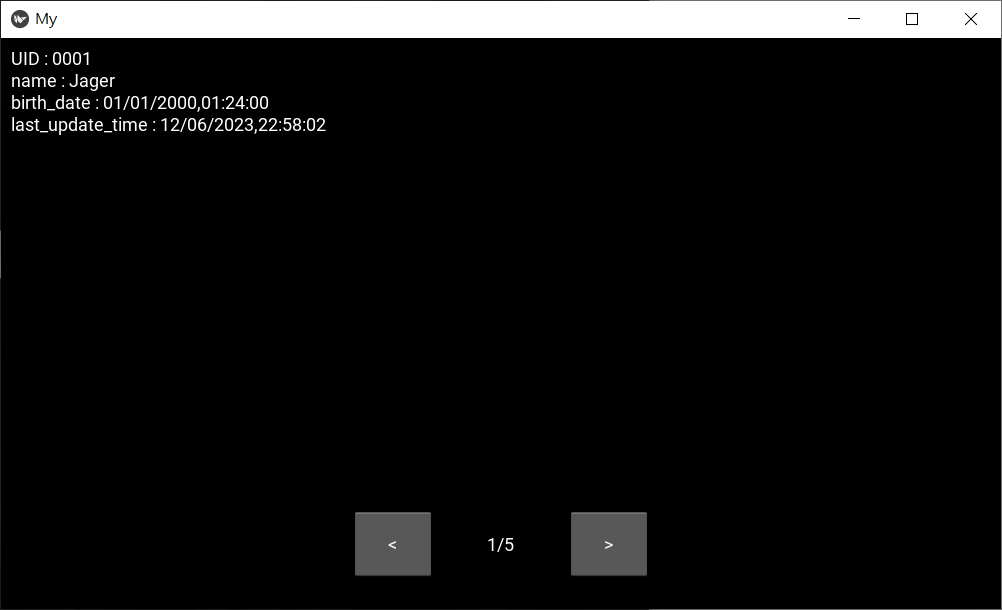
\includegraphics[scale = 0.4]{asset/doctor_gui/frontend_patient_info.png}
%  \caption{The prview of describe object}
%  \label{fig:frontend_patient_info}
%\end{figure}
The describe object will firstly process the info by using 
\codeword{process\_info(String)}, put it into a suitable format 
and divide it into parts. Then, it will present these information 
by using a scoll window, there are buttons to go prev and next 
pages, each pages present individual part of informations it 
just processed by \codeword{process\_info(String)}.

\subsubsection*{Reservation\_layout}

\begin{figure*}[htb]
  \vspace{\baselineskip}
  \begin{center}
      \begin{tabular}{cc}
          \subfigure[]{\resizebox{0.35\textwidth}{!}{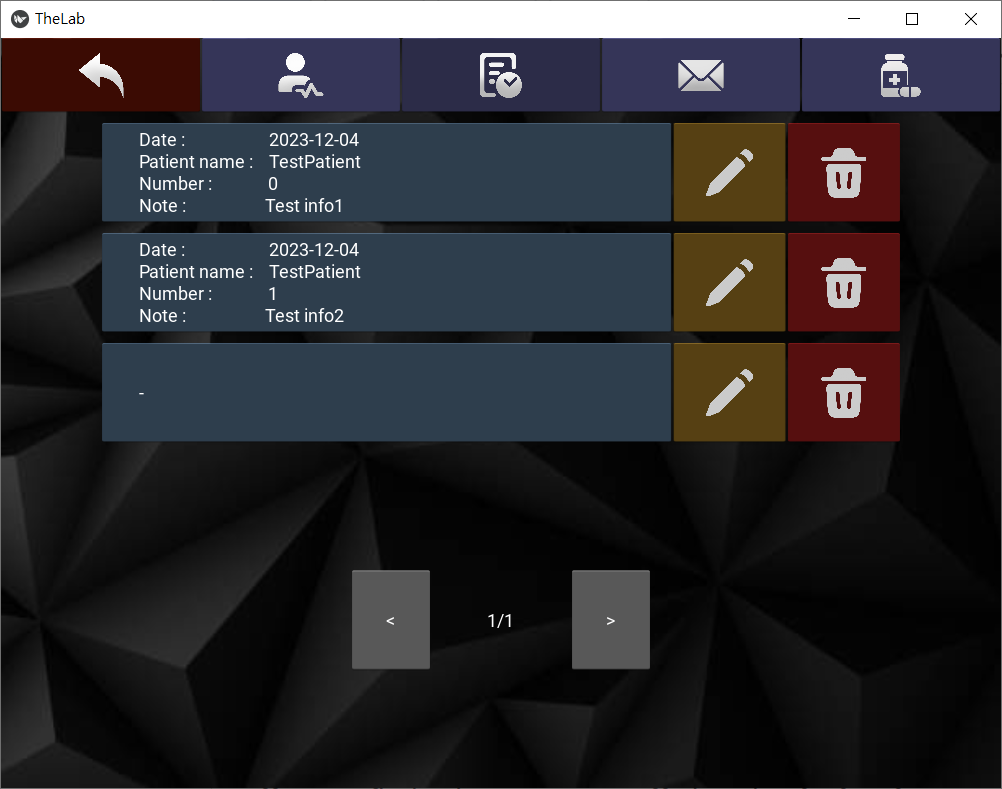
\includegraphics{asset/doctor_gui/frontend_reservation_browse.png}}}
          \subfigure[]{\resizebox{0.35\textwidth}{!}{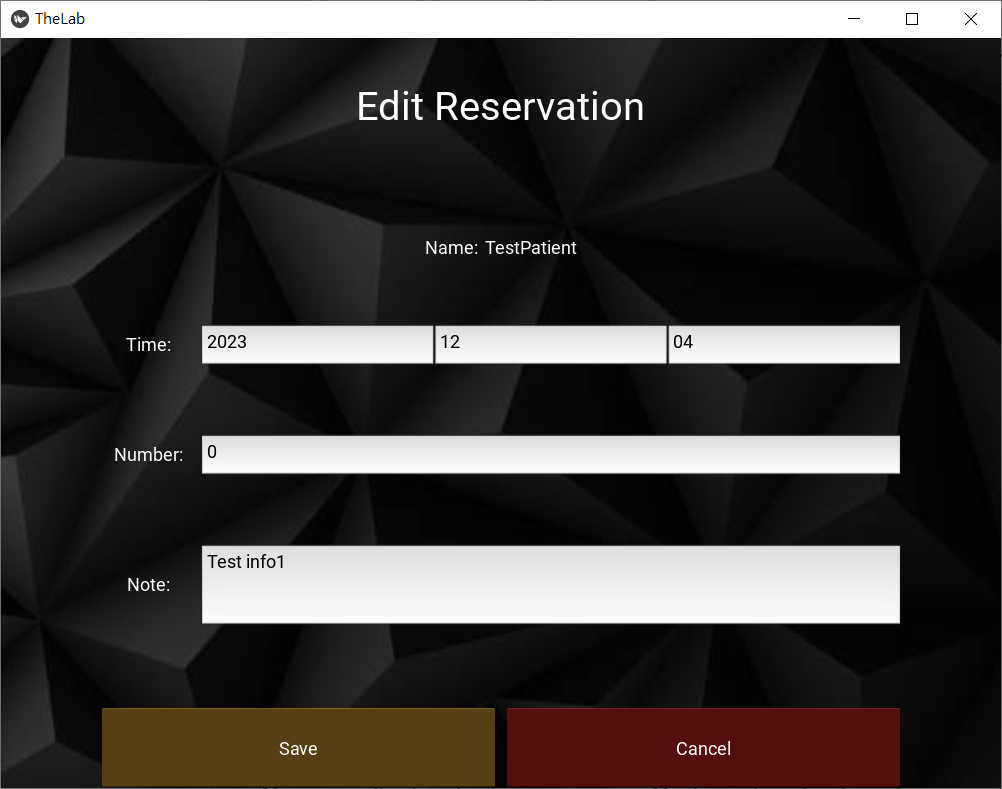
\includegraphics{asset/doctor_gui/frontend_reservation_edit.png}}}
      \end{tabular}
      \caption{(a) The prview of reservation\_layout 
      (b) The prview of EditResv}
      \label{fig:frontend_reservation_browse_edit}
  \end{center}
  \vspace{-\baselineskip}
\end{figure*}

Reservation will load the reservation objects of medium (linebot), 
divide it into multiple pieces, store them as attributes, and 
display it in the main window as an embedded page. Each piece of 
data will display the name of the reservation person, reservation 
time, reservation time and remarks. The button below can call the 
prev\_page and next\_page methods to browse other reservation 
information.

\begin{itemize}
  \item \codeword{delete\_resv():} Activated by the red trash can button. Will delete reservation the button belongs to from its own attributes, then will call \codeword{fix\_page()} to refresh the embedded page.
  \item \codeword{chg\_edit\_resv():} Activated by the yellow pen button. The method will change current page to \codeword{EditResv} class, doctor can edit the reservation the button belongs to. After press the save button the data will be stored to that reseravtion and called \codeword{change\_to\_Reservatoin()} to return to original page.
\end{itemize}

\subsubsection*{Chat\_layout}

\begin{figure*}[htb]
  \vspace{\baselineskip}
  \begin{center}
      \begin{tabular}{ccc}
          \subfigure[]{\resizebox{0.3\textwidth}{!}{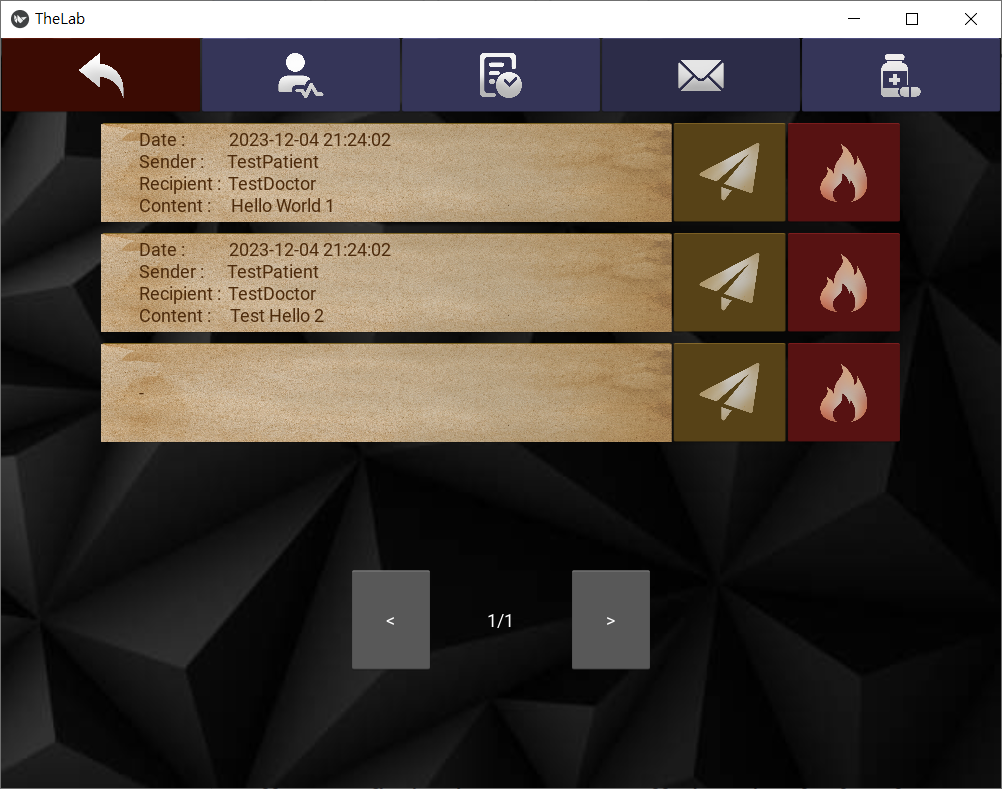
\includegraphics{asset/doctor_gui/frontend_chat_browse.png}}}
          \subfigure[]{\resizebox{0.3\textwidth}{!}{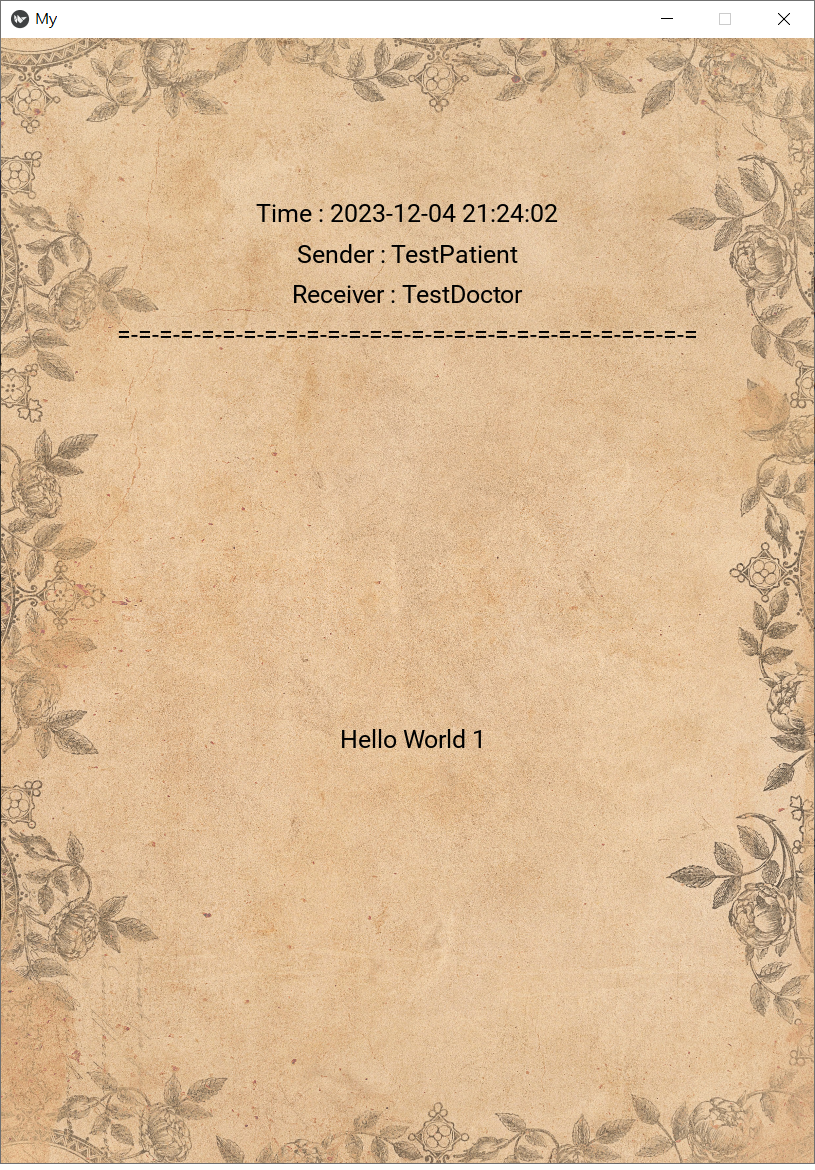
\includegraphics{asset/doctor_gui/frontend_chat_show.png}}}
          \subfigure[]{\resizebox{0.3\textwidth}{!}{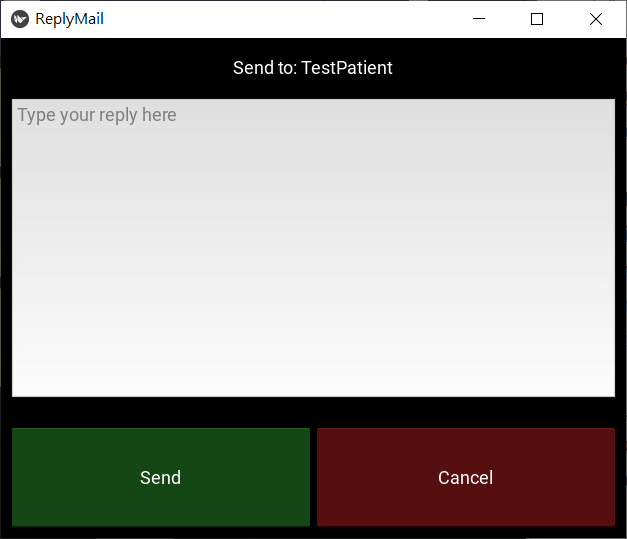
\includegraphics{asset/doctor_gui/frontend_chat_reply.png}}}
      \end{tabular}
      \caption{(a) The prview of Chat\_layout 
      (b) The prview of MailDisplay
      (c) The prview of ReplyMail}
      \label{fig:frontend_chat}
  \end{center}
  \vspace{-\baselineskip}
\end{figure*}

%\begin{figure}[h]
%  \centering
%  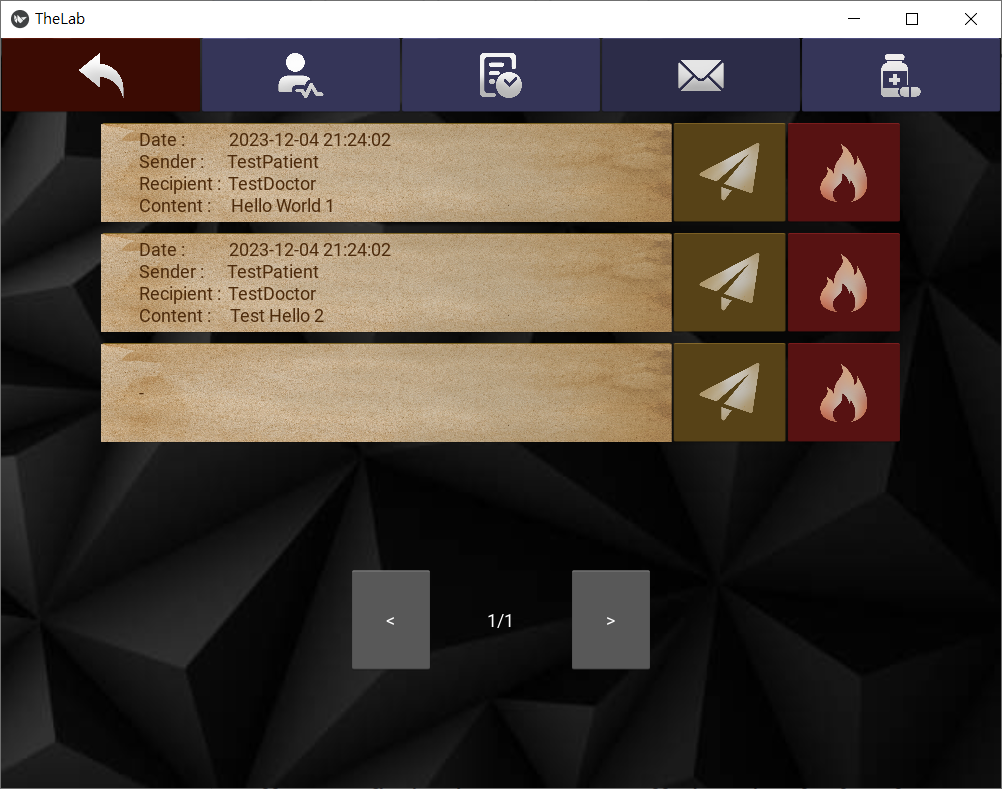
\includegraphics[scale = 0.4]{asset/doctor_gui/frontend_chat_browse.png}
%  \caption{The prview of Chat\_layout}
%  \label{fig:frontend_chat_browse}
%\end{figure}
The approach of Chat is very similar to that of Reservation. It will 
load the Message objects of medium (linebot), divide them into blocks, 
and display their summary on the embedded page. What is different from 
Reseravtion is the button part, which will be explained in detail below.

%\begin{figure}[h]
%  \centering
%  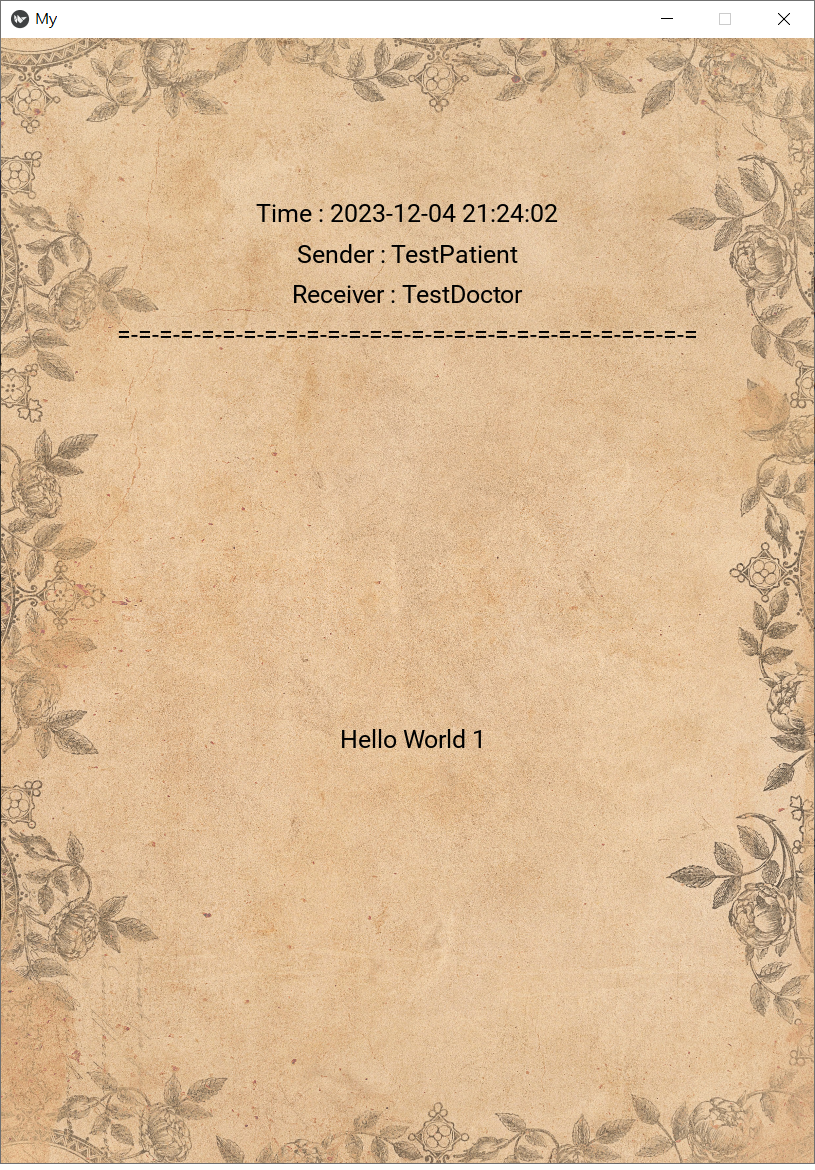
\includegraphics[scale = 0.4]{asset/doctor_gui/frontend_chat_show.png}
%  \caption{The prview of MailDisplay}
%  \label{fig:frontend_chat_show}
%\end{figure}
%\begin{figure}[h]
%  \centering
%  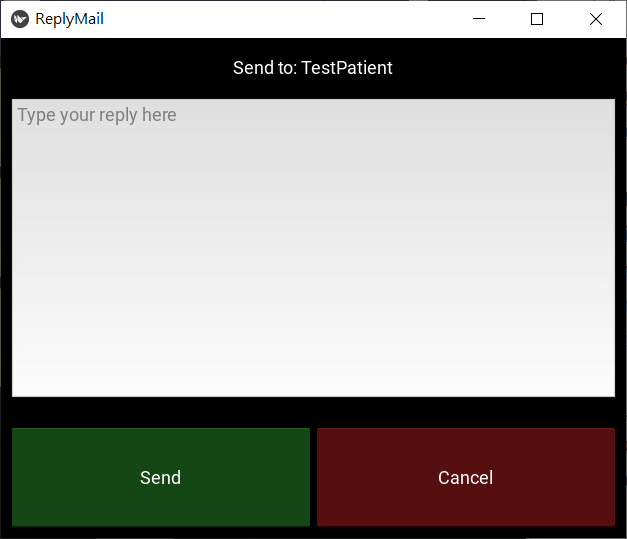
\includegraphics[scale = 0.4]{asset/doctor_gui/frontend_chat_reply.png}
%  \caption{The prview of ReplyMail}
%  \label{fig:frontend_chat_reply}
%\end{figure}

\begin{itemize}
  \item \codeword{check\_mail():} Activated by clicking the summary of that message. It will call a subprocess and passing needed arguments such as sender, date, message. Then the subprocess will display these information by \codeword{MailDisplay}.
  \item \codeword{delete\_mail():} Activated by the red fire button. Will delete message the button belongs to, then will call \codeword{fix\_page()} to refresh the embedded page.
  \item \codeword{reply\_mail():} Activated by the yellow paper airplane button. It will also call a subprocess to let doctor write message to the sender. After pressing save button, the message will be send to the sender by using \codeword{reply} method that the mail have defined in medium(linebot)'s \codeword{Message}.
\end{itemize}

\subsubsection*{Prscribe\_layout}
\begin{figure}[ht]
  \centering
  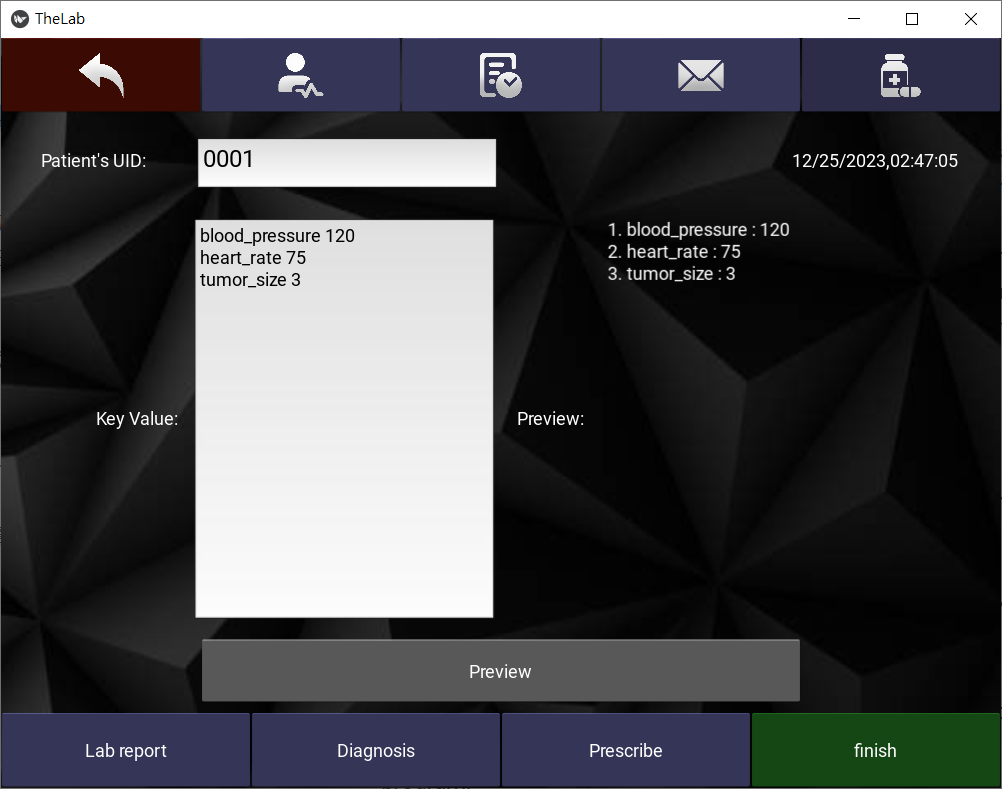
\includegraphics[scale = 0.3]{asset/doctor_gui/frontend_prescribe.png}
  \caption{The prview of Prescibe\_layout}
  \label{fig:frontend_prescribe}
\end{figure}

Doctors can create/attach prescription to speific patient such as associative 
data, lab report or diagonosis. The following will introduce the functions of 
each method and button in detail.

\begin{itemize}
  \item \codeword{update\_scollview():} Activated by the preview button. Will load the textinput right of "Key Value:" text, process them into proper format and update the scroll window right of "Preview:" text. The reason to create such a function like this is cause associative values are strictly format, doctors can preview the result to check if there is something wrong by this method.
  \item \codeword{open\_...():} Several methods behave very similarly. They all start a subprocess to allow doctors to edit data and store it in their corresponding attrubute.
  \item \codeword{finish():} After all the data has been edited, press the finish button to call. First, the function will search for the corresponding patient based on the entered UID. If it is found, it will directly load the patient's information (\codeword{patient\_info\_t}). If the patient cannot be found, the program will first ask the doctor to create a file for the patient. Next, save all the entered data into a new \codeword{reports\_t} object, then save \codeword{reports\_t} into a new \codeword{med\_record\_t} object, append the data into the \codeword{patient\_info\_t} object just loaded or created, and finally save the updated \codeword{patient\_info\_t} to database
\end{itemize}

\section{Code}
\label{sec:code}
All the code can be found \href{https://github.com/OEmiliatanO/E-health}{here}.

\section{Conclusion}
\label{sec:conclusion}
In this project, we develope a E-healthcare management system, which solves 
the syncing problem between different health systems by using local and 
central database, and facilitate most of the services by transfer them into 
internet. Even more, we introduce the automatic disease detectors, which 
is able to detect multiple diseases by leveraging the machine learning 
techniques. 

In technological aspect, we use object-oriented programming to shorten the 
development time, and modularize the whole system into several parts, like 
database, frontend, medium, and detector (processor). With that, the system 
is highly scalable and easy to maintain. 

\section{Contribution}
\label{sec:contribution}

\begin{itemize}
  \item \texttt{B103040012} (Cheng-Han Hsieh, 謝承翰): the architecture of system, database, paper report
  \item \texttt{B103040001} (Shih-Yu Sun, 孫世諭): medium, frontend, linebot, coordination and communication, paper report
  \item \texttt{B103040051} (Chia-Huang, 黃嘉彥): Doctor GUI(include design, data process, images, code), paper report
  \item \texttt{B103040008} (Ting-Hao Hsu, 許廷豪): Preprocessor and Detector, paper report
  \item \texttt{B093040051} (Casper Liu, 劉世文): visualization of the architecture, presentation
  \item \texttt{B096060032} (Tina Tsou, 鄒宜庭): visualization of the architecture, presentation
\end{itemize}
\end{document}